\chapter{}
\section{Вступні відомості}
\noindent\textbf{Мета роботи:} Ознайомлення з принципами баєсівського підходу в криптоаналізі, побудова детерміністичної та стохастичної 
вирішуючих функцій для моделей схем шифрування та криптоаналіз моделей шифрів за допомогою програмної реалізації, зокрема здійснення 
порвіняльного аналізу вирішуючих функцій.

\noindent\textbf{Постановка задачі:}
\begin{enumerate}
    \item Створіть репозиторій у системі контролю версій Git/GitHub;
    \item Реалізуйте алгоритми програмно та представите результати побудови детермінованих та стохастичних вирішальних функцій у 
        вигляді таблиць. Для цього необхідно:
        \begin{enumerate}
            \item обчислити розподіли $P(C)$ та $P(M, C)$;
            \item на основі цих розподілів обчислити $P(M \vert C)$;
            \item побудова оптимальних детермінованих та стохастичних вирішальних функцій зводиться до максимізації $P(M \vert C)$.
        \end{enumerate}
    \item Розрахуйте середні втрати, проведіть порівняльний аналіз функцій прийняття рішень.
    \item Підготувати звіт для комп'ютерного практикуму.
\end{enumerate}
\section{Результати виконання роботи. Варіант 15}
\begin{figure}[!ht]
    \centering
    \begin{minipage}{0.6\linewidth}
        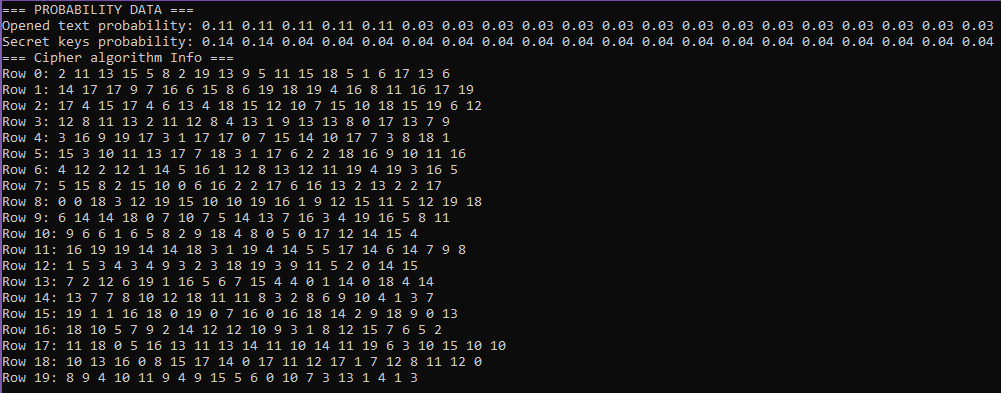
\includegraphics[width=0.6\textwidth, scale=0.05]{ReportPic/report_1.png}
    \end{minipage}
\end{figure}
\newpage
\begin{figure}[!ht]
    \centering
    \begin{minipage}{0.35\linewidth}
        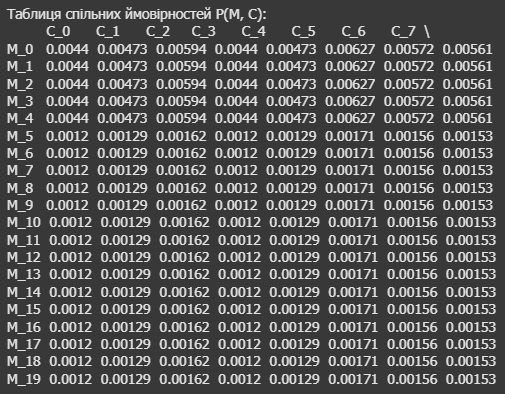
\includegraphics[width=0.85\textwidth]{ReportPic/report_2.1.png}
    \end{minipage}
    \begin{minipage}{0.35\linewidth}
        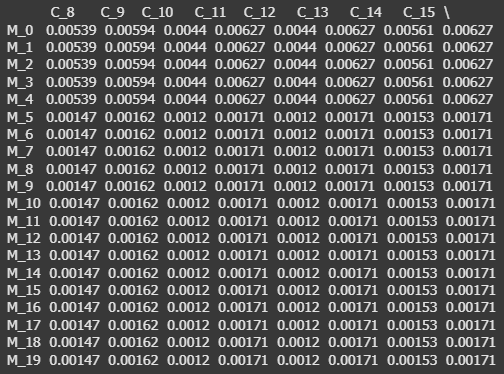
\includegraphics[width=0.85\textwidth]{ReportPic/report_2.2.png}
    \end{minipage}
    \begin{minipage}{0.25\linewidth}
        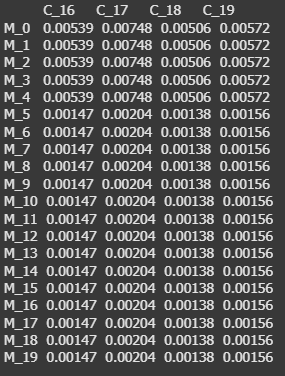
\includegraphics[width=0.85\textwidth]{ReportPic/report_2.3.png}
    \end{minipage}
\end{figure}
\begin{figure}[!ht]
        \centering
        \begin{minipage}{0.55\linewidth}
            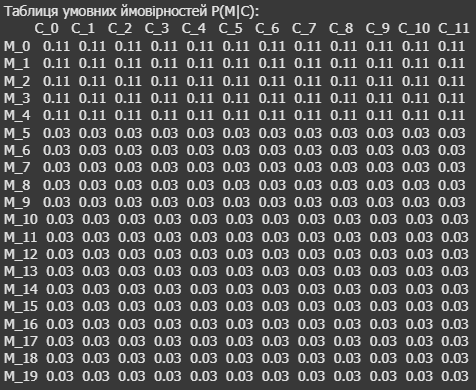
\includegraphics[width=0.8\textwidth, scale=0.6]{ReportPic/report_3.1.png}
        \end{minipage}
        \begin{minipage}{0.4\linewidth}
            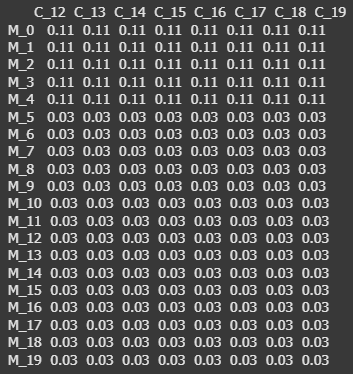
\includegraphics[width=0.8\textwidth, scale=0.5]{ReportPic/report_3.2.png}
        \end{minipage}
\end{figure}
\section{Побудова вирішуючих функцій}
\begin{definition}    
    ~\par Оптимальна (баєсівська) детерміністична функція [в межах лабораторної роботи] визначається наступним чином: 
    \begin{equation*}
        \delta_{B} = \left\{\delta_{B}^{(n)} : \mathcal{M} \rightarrow \mathcal{C}\right\}, 
    \end{equation*}
    де $P \left(\delta_{B}^{(optim)} \vert C\right) = \max\limits_{m \in M} P \left(M_{i} \vert C\right)$. \\ 
    Тобто фактично детерміністична функція дорівнює довільному шифротексту, який дорівнює максимальному значенню в 
    $i$-тому рядку таблиці.
\end{definition}
\begin{definition}
    ~\par Стохастична розв'язувальна функція $\delta_{D}$ є оптимальною тоді і тільки тоді, коли $\forall \, n$ 
    з нерівності $\delta_{c}^{(n)} \left(C, M\right) > 0$ випливає, що $P \left(M \vert C\right) = \max\limits_{M'} P \left(M' \vert C\right)$.
    Тобто 
    \begin{equation*}
        \delta_{D}^{optim} \left(C, m\right) = 
        \begin{cases}
            \frac{1}{\vert M \vert}, \text{ if } P \left(M \vert C\right) = \max\limits_{M'} P \left(M' \vert C\right) \\
            0, \text{ otherwise}
        \end{cases}
    \end{equation*}
\end{definition}
\newpage

\begin{figure}[!ht]
    \centering
    \begin{minipage}{0.85\linewidth}
        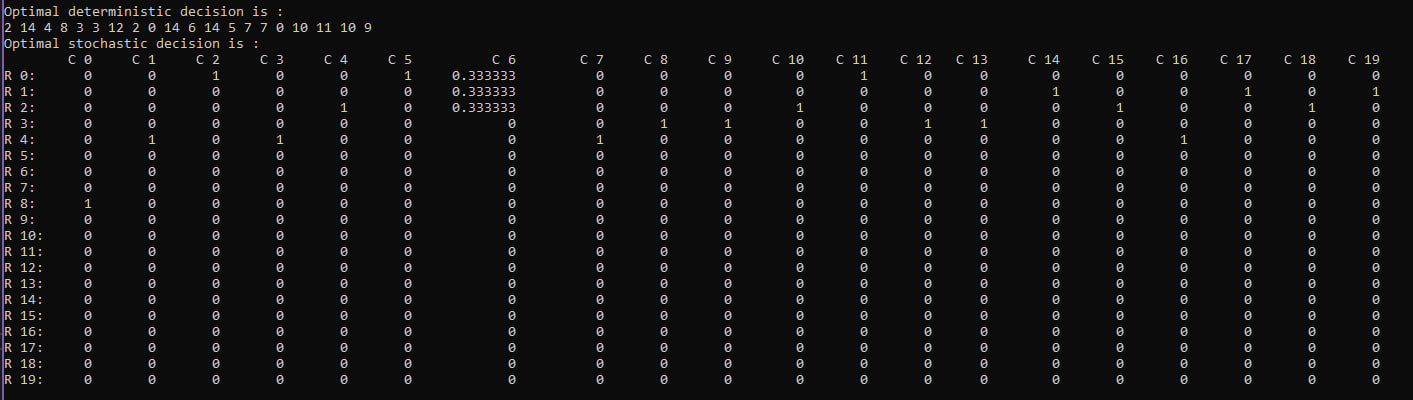
\includegraphics[width=0.5\textwidth, scale=0.2]{ReportPic/report_4.png}
    \end{minipage}
\end{figure}

Як результат роботи - видало перший ліпший $M_{i}$ (за критеріями підходить декілька)
\begin{figure}[!ht]
        \centering
        \begin{minipage}{0.55\linewidth}
            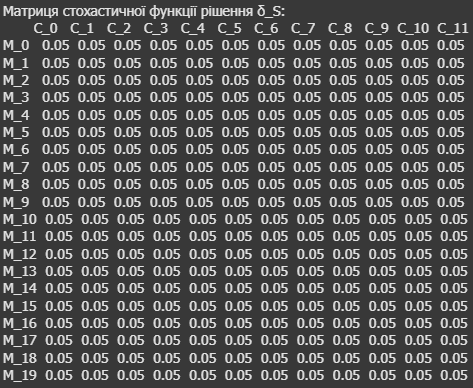
\includegraphics[width=0.8\textwidth, scale=0.6]{ReportPic/report_5.1.png}
        \end{minipage}
        \begin{minipage}{0.4\linewidth}
            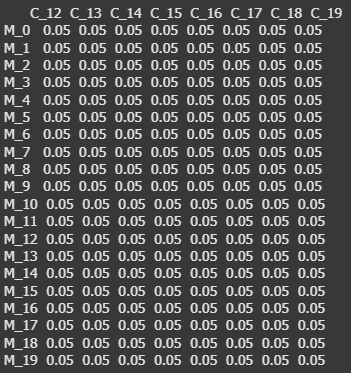
\includegraphics[width=0.8\textwidth, scale=0.5]{ReportPic/report_5.2.png}
        \end{minipage}
\end{figure}
\begin{figure}[!ht]
        \centering
        \begin{minipage}{0.55\linewidth}
            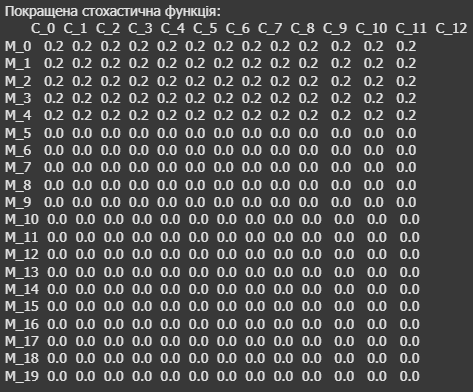
\includegraphics[width=0.8\textwidth, scale=0.6]{ReportPic/report_6.1.png}
        \end{minipage}
        \begin{minipage}{0.4\linewidth}
            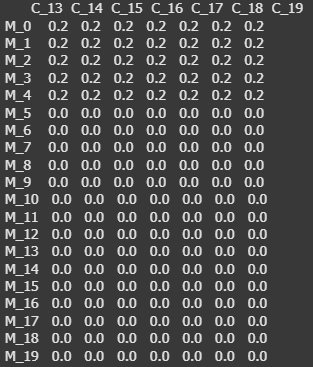
\includegraphics[width=0.8\textwidth, scale=0.5]{ReportPic/report_6.2.png}
        \end{minipage}
\end{figure}
\begin{figure}[!ht]
        \centering
        \begin{minipage}{0.85\linewidth}
            
\includegraphics[width=0.8\textwidth, scale=0.6]{ReportPic/report_7.1.png}
        \end{minipage}
        \begin{minipage}{0.85\linewidth}
            
\includegraphics[width=0.8\textwidth, scale=0.5]{ReportPic/report_7.2.png}
        \end{minipage}
\end{figure}

\section{Висновки:}
Подивившись на отримані результати середніх втрат можна впасти в ступор, оскільки вони виявилися однаковими. На нашу думку це 
може бути бути пов'язано з недостатньою точністю обрахунків. Маємо припущення, що стохастична (a.k.a. випадкова) вирішуюча 
функція мала б відповідати більшій кількості потенційних ВТ до відповідно обраного ШТ, порівняно зі строго детерміністичною. 
Вона також могла показувати як зашкально добрий результат, так і навпаки (жартуємо, будь-яку випадковість можна передбачити). 
Варто зазначити, що при збільшенні кількості вхідних даних, стохастична вирішуюча функція (яка являє собою багаторозмірну 
матрицю) буде займати багатенько пам'яті, що може сповільнити процес виконання програми.